\subsection{Learning Statistics}

\subsubsection{Learning Process}

Figure (\ref{fig:first_traning_cycle}) and (\ref{fig:second_traning_cycle}) shows the Mean Squared Error (MSE) during the first and second training cycles for the DICE 2016 and DICE 2023 variations of ACE. Initially, in the first training cycle, both policy networks exhibit a high MSE, which quickly decreases as the number of iterations progresses. This rapid error reduction indicates that the model correctly adjusts to the learning signals and aligns with what I would expect from the early training iterations.

Throughout the first training cycle, the MSE for both policy networks generally trends downward, suggesting improvements in accuracy. Comparatively, the training of the policy network for the DICE 2016 version displays a more rapid fall in errors and seems to get closer to convergence than the DICE 2023 version. However, there are notable spikes in MSE for both models. 

\begin{figure}[H]
  \centering
  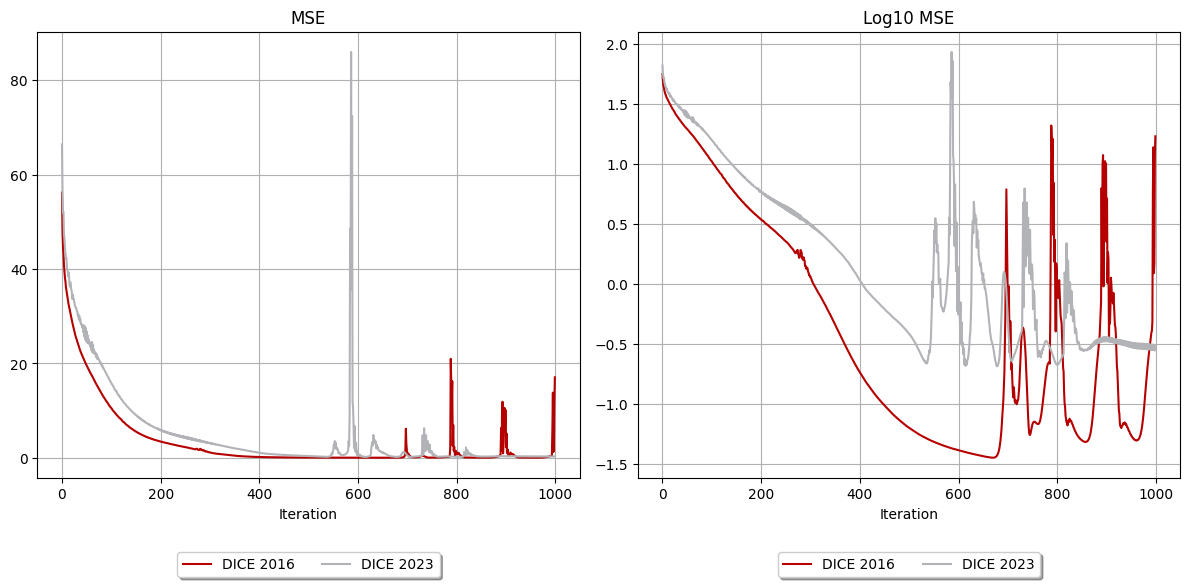
\includegraphics[width=1.0\textwidth]{images/ch6/errors over iterations/JOINT PLOT, run 1, 1e-4, 1000 iterations, ep length 64, batch size 32.png}
  \caption{First training cycle learning statistics}
  \label{fig:first_traning_cycle}
\end{figure}

The outcomes from the second training cycle resemble the last part of the first training cycle. Both policy networks continue to demonstrate variability in MSE. Notably, the 2016 version exhibits slightly more frequent fluctuations than the 2023 version, but the 2016 version achieves lower errors overall and has smaller spikes. 

Moreover, I would like to highlight that during the initial iterations of the second training cycle, the MSE for the 2023 version surged, exceeding 20,000. This surge in error also leads to exploding gradients, which are particularly problematic as they could completely derail the learning process. 

\begin{figure}[H]
  \centering
  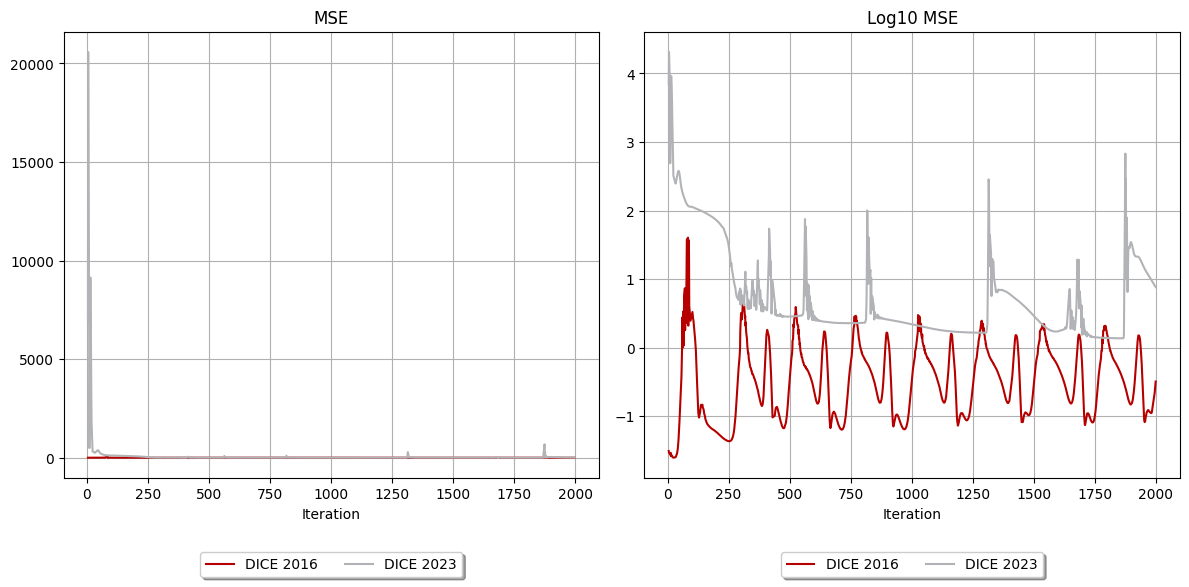
\includegraphics[width=1.0\textwidth]{images/ch6/errors over iterations/JOINT PLOT, run 2, 1e-4, 2000 iterations, ep length 128, batch size 128.png}
  \caption{Second training cycle learning statistics}
  \label{fig:second_traning_cycle}
\end{figure}


\subsubsection{Errors in Equilibrium conditions}

The errors in the individual components that make up the total objective function, as given in equation (\ref{eq:total_objective_function}), are presented in tables (\ref{table:errors2016}) and (\ref{table:errors-2023}). The statistics presented in each column show the absolute errors \(|\ell_m|\) for the respective Lagrange condition over an episode generated with the best-performing model from the last training cycles.


\begin{table}[H]
\centering
\begin{adjustbox}{width=\textwidth,center}
{
% PASTE RESULTS HERE
\begin{tabular}{lrrrrrrrrrrr}
\toprule
Statistic & \(\ell_0\) (\ref{eq:general_objective_0}) & \(\ell_{1,M_1}\) (\ref{eq:general_objective_1}) & \(\ell_{1,M_2}\) (\ref{eq:general_objective_1}) & \(\ell_{1,M_3}\) (\ref{eq:general_objective_1}) & \(\ell_{2,\tau_1}\) (\ref{eq:general_objective_2}) & \(\ell_{2,\tau_2}\) (\ref{eq:general_objective_2}) & \(\ell_3\) (\ref{eq:general_objective_3}) & \(\ell_4\) (\ref{eq:general_objective_4}) & \(\ell_{5, A}\) (\ref{eq:general_objective_5}) & \(\ell_{5,B}\) (\ref{eq:ell_5B_FB-E_t^BAU}) & \(\ell_6\) (\ref{eq:general_objective_6}) \\
\midrule
mean & 0.096164 & 0.000371 & 0.000966 & 0.002724 & 0.001815 & 0.001568 & 0.030191 & 0.002744 & 0.004898 & 0.006045 & 0.084397 \\
std & 0.010226 & 0.000389 & 0.000580 & 0.001392 & 0.001251 & 0.001006 & 0.026208 & 0.003337 & 0.002683 & 0.005978 & 0.088106 \\
min & 0.013111 & 0.000004 & 0.000009 & 0.000033 & 0.000018 & 0.000011 & 0.000307 & 0.000016 & 0.000028 & 0.000047 & 0.000130 \\
0.1\% & 0.016954 & 0.000004 & 0.000014 & 0.000043 & 0.000019 & 0.000012 & 0.000308 & 0.000017 & 0.000028 & 0.000056 & 0.000317 \\
25\% & 0.096827 & 0.000084 & 0.000538 & 0.001633 & 0.000524 & 0.000716 & 0.010575 & 0.000709 & 0.002647 & 0.001837 & 0.026514 \\
50\% & 0.097503 & 0.000311 & 0.000932 & 0.002781 & 0.001832 & 0.001442 & 0.023612 & 0.001934 & 0.005039 & 0.003853 & 0.057354 \\
75\% & 0.100176 & 0.000530 & 0.001346 & 0.003942 & 0.002943 & 0.002301 & 0.036951 & 0.003536 & 0.006983 & 0.008398 & 0.119186 \\
99.9\% & 0.101675 & 0.002086 & 0.003015 & 0.007022 & 0.004592 & 0.003733 & 0.101944 & 0.019297 & 0.011890 & 0.025575 & 0.471371 \\
max & 0.101678 & 0.002100 & 0.003067 & 0.007337 & 0.004663 & 0.003736 & 0.102000 & 0.019462 & 0.012184 & 0.025795 & 0.474888 \\
\bottomrule
\end{tabular}
% END PASTE HERE
}
\end{adjustbox}
\caption{Error Statistics ACE-DICE (2016 DICE)}
\label{table:errors2016}
\end{table}

In Table (\ref{table:errors2016}), the largest errors for the 2016 version seem to be on the Lagrange condition for capital \(\ell_0\), the consumption rate \(\ell_3\), and the Bellman equation \(\ell_6\), where the Bellman equation has the most extreme errors. Generally, the conditions on the carbon reservoirs \(\ell_1\) and temperatures \(\ell_2\) seem to give lower errors. None of the error statistics in this table reaches the levels reported in \textcite{Folini2024ClimateInCE}. It is impossible to compare with the errors of the policy network in \textcite{friedl2023_deepUQ} as they do not report them.

\begin{table}[H]
\centering
\begin{adjustbox}{width=\textwidth,center}
{
% PASTE RESULTS HERE
\begin{tabular}{lrrrrrrrrrrr}
\toprule
Statistic & \(\ell_0\) (\ref{eq:general_objective_0}) & \(\ell_{1,M_1}\) (\ref{eq:general_objective_1}) & \(\ell_{1,M_2}\) (\ref{eq:general_objective_1}) & \(\ell_{1,M_3}\) (\ref{eq:general_objective_1}) & \(\ell_{2,\tau_1}\) (\ref{eq:general_objective_2}) & \(\ell_{2,\tau_2}\) (\ref{eq:general_objective_2}) & \(\ell_3\) (\ref{eq:general_objective_3}) & \(\ell_4\) (\ref{eq:general_objective_4}) & \(\ell_{5, A}\) (\ref{eq:general_objective_5}) & \(\ell_{5,B}\) (\ref{eq:ell_5B_FB-E_t^BAU}) & \(\ell_6\) (\ref{eq:general_objective_6}) \\
\midrule
mean & 0.001079 & 0.002681 & 0.002797 & 0.001330 & 0.003702 & 0.002662 & 0.090005 & 0.012109 & 0.007052 & 0.000345 & 0.942334 \\
std & 0.001487 & 0.007117 & 0.001938 & 0.001367 & 0.002522 & 0.002140 & 0.067977 & 0.009595 & 0.005061 & 0.000211 & 0.687683 \\
min & 0.000003 & 0.000002 & 0.000100 & 0.000009 & 0.000136 & 0.000002 & 0.000419 & 0.000041 & 0.000061 & 0.000000 & 0.013466 \\
0.1\% & 0.000004 & 0.000006 & 0.000105 & 0.000009 & 0.000138 & 0.000005 & 0.000467 & 0.000045 & 0.000062 & 0.000000 & 0.014943 \\
25\% & 0.000514 & 0.000683 & 0.001746 & 0.000403 & 0.002205 & 0.001127 & 0.040442 & 0.005515 & 0.003632 & 0.000122 & 0.509475 \\
50\% & 0.000808 & 0.001661 & 0.002235 & 0.000829 & 0.002672 & 0.002323 & 0.083141 & 0.008511 & 0.005676 & 0.000395 & 0.994534 \\
75\% & 0.001289 & 0.003195 & 0.002961 & 0.001464 & 0.004958 & 0.003550 & 0.123408 & 0.017240 & 0.009491 & 0.000522 & 1.336148 \\
99.9\% & 0.014170 & 0.070844 & 0.008989 & 0.005521 & 0.010437 & 0.012418 & 0.339296 & 0.046774 & 0.021824 & 0.000612 & 6.011588 \\
max & 0.015410 & 0.080187 & 0.009035 & 0.005528 & 0.010483 & 0.012866 & 0.345071 & 0.048375 & 0.022131 & 0.000613 & 6.647907 \\
\bottomrule
\end{tabular}
% END PASTE HERE
}
\end{adjustbox}
\caption{Error Statistics ACE-DICE (2023 DICE)}
\label{table:errors-2023}
\end{table}

The most notable error in Table (\ref{table:errors-2023}) are the errors in the Bellman equation \(\ell_6\), reaching a maximum absolute error of approximately 6.648. The second highest errors are observed in the Lagrange condition for the consumption rate \(\ell_3\). The policy network also struggles to learn the Lagrange condition on emissions \(\ell_4\). Similar to the 2016 version, the conditions on the carbon reservoirs \(\ell_1\) and temperatures \(\ell_2\) also give lower errors here. These error statistics did also not reach the low errors reported in \textcite{Folini2024ClimateInCE}.


\subsubsection{Discussion on Learning Statistics}

The model's failure to converge could be attributed to inadequate normalization of the input variables, which hindered proper learning and led to large gradients in this specific context. This issue is likely reflected by the significant fluctuations in the MSE shown in Figure (\ref{fig:first_traning_cycle}).

While the Adam optimizer is designed to mitigate issues arising from variable gradient scales through its adaptive learning rate mechanism, it can still struggle under large variations in scale among input features and, therefore, gradients. The optimizer's continual adaptation of learning rates based on the incoming gradients might also contribute to the observed spikes in MSE.
